\documentclass[11pt,letterpaper]{article}
\usepackage[T1]{fontenc}
\usepackage[utf8]{inputenc}
\usepackage[margin=1in,headheight=15pt]{geometry}
\usepackage{amsmath,amsthm,mathtools,newtxtext,newtxmath,microtype}
\usepackage{booktabs,tabularx,longtable,array,enumitem}
\usepackage{algorithm,algpseudocode,tikz,pgfplots,xcolor,fancyhdr,titlesec,needspace,placeins}
\usetikzlibrary{arrows.meta,positioning,calc,fit,backgrounds}
\pgfplotsset{compat=1.18}
\usepackage{xurl,hyperref,listings}
\definecolor{ink}{HTML}{35214E}
\definecolor{pale}{HTML}{F4F1F8}
\definecolor{muted}{HTML}{68616F}
\hypersetup{colorlinks=true,linkcolor=ink,citecolor=ink,urlcolor=ink,
 pdftitle={The World as an Output: Constructive Sufficiency for Reusable Discovery},
 pdfauthor={Vincent Boucher},pdfsubject={Purpose-preserving system construction, unknown nuisance dynamics, sharp repeatability costs, and successor capabilities}}
\urlstyle{same}
\pagestyle{fancy}\fancyhf{}
\fancyhead[L]{\small\textsc{The World as an Output}}\fancyhead[R]{\small Boucher}\fancyfoot[C]{\thepage}
\renewcommand{\headrulewidth}{.3pt}
\setlength{\parindent}{1.1em}\setlength{\parskip}{.18em}\setlength{\emergencystretch}{2em}
\setlength{\tabcolsep}{4.5pt}\renewcommand{\arraystretch}{1.13}
\setlist{nosep,leftmargin=1.5em,topsep=.3em}
\titleformat{\section}{\large\bfseries\color{ink}}{\thesection}{.6em}{}
\titleformat{\subsection}{\normalsize\bfseries}{\thesubsection}{.6em}{}
\titlespacing*{\section}{0pt}{1.25em}{.5em}\titlespacing*{\subsection}{0pt}{.8em}{.3em}
\newcolumntype{Y}{>{\raggedright\arraybackslash}X}
\newcolumntype{P}[1]{>{\raggedright\arraybackslash}p{#1}}
\newtheorem{theorem}{Theorem}[section]
\newtheorem{proposition}[theorem]{Proposition}
\newtheorem{corollary}[theorem]{Corollary}
\newtheorem{lemma}[theorem]{Lemma}
\theoremstyle{definition}\newtheorem{definition}[theorem]{Definition}
\theoremstyle{remark}\newtheorem{remark}[theorem]{Remark}
\newcommand{\R}{\mathbb R}\newcommand{\N}{\mathbb N}\newcommand{\one}{\mathbf1}
\newcommand{\supp}{\operatorname{supp}}\newcommand{\Post}{\operatorname{Post}}
\newcommand{\Om}{SUCCESSOR $\Omega$}
\newcommand{\insight}[1]{\begin{center}\setlength{\fboxsep}{8pt}\fcolorbox{ink}{pale}{\begin{minipage}{.93\linewidth}#1\end{minipage}}\end{center}}
\lstset{basicstyle=\small\ttfamily,breaklines=true,columns=fullflexible,keepspaces=true,showstringspaces=false,frame=single,rulecolor=\color{muted}}
\renewcommand{\topfraction}{.95}\renewcommand{\bottomfraction}{.85}\renewcommand{\textfraction}{.06}\renewcommand{\floatpagefraction}{.8}
\begin{document}
\thispagestyle{plain}
\begin{center}
{\small\textsc{MONTREAL.AI\quad /\quad Transformational Intelligence}\par}
\vspace{.9em}
{\fontsize{30}{34}\selectfont\bfseries\color{ink} The World as an Output\par}
\vspace{.6em}
{\Large Constructive Sufficiency for Reusable Discovery\par}
\vspace{1em}
{\large Vincent Boucher\par}
MONTREAL.AI\par
Montr\'eal, Qu\'ebec, Canada\par
\vspace{.5em}
20 October 2026\quad$\cdot$\quad Research manuscript
\end{center}
\begin{abstract}
An intelligence can spend its resources reconstructing hidden conditions that a different productive system would make irrelevant. We investigate the latter possibility: construct an experimental interface that preserves the intended work while removing its dependence on nuisance dynamics. The output is a reusable capability, not an estimate of the entire world. We give an executable constructor for guarded nonnegative systems with unknown, potentially time-varying coefficients. A necessary-and-sufficient support criterion determines whether a construction protects an entire language of future operations, rather than only the first readout. A weighted compiler returns a least-cost protected program, its installation requirements, and an independently checkable optimality certificate within the stated catalogue. For imperfect preparation, a second result gives a sharp, history-uniform error envelope under a declared recurring disturbance contract. A third result derives the exact local actuation cost of meeting that contract in a cyclic architecture: consecutive attenuation operations at each visited location are optimal, and repeated full sweeps can be unnecessarily expensive. In the executed six-channel case, a protocol passes its first accuracy test but fails on its second use. The recurrent construction remains within a $0.0005$ error requirement and uses 30 abstract operation units rather than 50 for repeated sweeps. Exact replay covers 8,192 adaptively chosen synthetic queries, two distinct downstream decision problems, 96 fresh structural systems, and a successor that activates a previously irrelevant reservoir. Commercial scope changes the infrastructure selected; profitability, finance and voluntary adoption remain separate obligations. The work constructs and tests an interface under supplied structural bounds. It does not claim unknown-law discovery, physical validation, autonomous business creation, or superiority over unrestricted engineering.
\end{abstract}
\noindent\textbf{Keywords:} transformational intelligence; capability synthesis; nuisance decoupling; repeatability; robust interfaces; successor construction; \Om.
\begin{center}\small\textbf{Find your Alpha. Build your SUCCESSOR $\Omega$.}\par
\href{https://github.com/MontrealAI/AGI-Alpha-Agent-v0}{github.com/MontrealAI/AGI-Alpha-Agent-v0}
\end{center}
\clearpage

\section{Do not require the solver to understand what the system can remove}
A research instrument returns a different result depending on what happened before the current experiment. Several hidden channels retain carryover. Their couplings drift. A powerful investigator could try to reconstruct every residual, estimate every coupling and correct every reading. A larger community of agents could share that work. Neither arrangement eliminates its recurring cause.

A different objective is to construct an interface under which the experiment no longer depends materially on those hidden conditions. The useful specimen, design variables and intended scientific question must survive unchanged. Only a nuisance dependency may be removed. The resulting asset is not another model of carryover. It is a way to perform a family of experiments without reconstructing carryover each time.

This distinction is the central move of the paper. The preceding manuscript, \emph{Discoverability by Construction}, compiled new measurement programs from known finite primitive maps \cite{boucherD}. It made missing experimental access an output, but assumed that each population could be freshly prepared and that primitive meanings were known. The present construction makes a qualified preparation interface an output and replaces exact numerical dynamics with structural and magnitude envelopes. Unknown productive response functions remain outside the constructor. They are investigated through the interface after it has been constructed.

\insight{\textbf{An enabling capability can remove a prerequisite for inference.}\par\smallskip Instead of requiring extraordinary intelligence to control an opaque process, construct a process whose unwanted hidden dependencies cannot affect the authorized work---or affect it only within an explicit, reusable bound.}

\subsection{A concrete change in the object of invention}
The main synthetic apparatus has six nuisance channels and a seventh dormant reservoir. A local drain can clear one channel. An unguided mixer can propagate an unknown channel into either neighbor. A protective interlock preserves the workpiece during maintenance. An optional directional guide changes which transfers are possible. The constructor selects installations and composes primitive operations; it is not handed a completed cleaning program.

Three complications make an isolated successful readout inadequate. First, a hidden channel that is harmless now can become visible after later operations. Second, real attenuation need not be a perfect reset: residuals and new contamination can accumulate. Third, a later service can introduce a new operation that exposes the dormant reservoir. A capability must therefore carry its future-operation scope, recurring error contract and explicit extension rule.

For the reference precision requirement, two local attenuations per channel are enough for the first experiment. They are not enough for repeated experiments. Three per channel meet the recurring contract. The compiler's local construction batches those attenuations before moving to another channel. It avoids the extra routing of three complete sweeps and has a matching lower bound on operation cost. The numerical difference is modest enough to inspect; the logical difference is more important: the accepted service obligation changes what must be built.

\subsection{What is new, and what is not}
The contribution has three connected parts. The first is \emph{purpose-closed construction}: eliminate nuisance influence on every finite composition in a declared productive language, while preserving a protected state. The second is \emph{repeatability by construction}: turn a recurring disturbance budget into a qualified, optimally scheduled local interface rather than treating a successful first use as evidence of indefinite reliability. The third is \emph{executable succession}: detect when a new operation invalidates the old scope and synthesize the missing protected extension.

Nonnegative matrix mortality, synchronization, disturbance decoupling, shortest paths and robust refinement are established fields \cite{ryzhikov,kiefer,vorel,willems,reissig}. We do not rename them as inventions. The new results here specify the purpose-closed and recurring contracts, derive their exact consequences for the constructed architecture, and connect an executed constructor, lower bounds, failure witnesses and commercial scope. A specialist using the same mathematics can match the reference optima. No exhaustive priority claim is made for every lemma.

The underlying physical support restrictions, actuator envelopes and preservation guarantees are supplied. The code discovers programs within those restrictions, not the laws that justify them. In particular, ``unknown dynamics'' means unknown numerical coefficients, initial conditions and allowed drift inside a stated class. It does not mean an unconstrained unknown universe.

\section{Separate the useful work from the nuisance}
\label{sec:model}
\subsection{The protected purpose and the operations}
Let $x\in\mathcal X$ denote a protected specimen or productive state, $h\in\R_+^d$ a nuisance vector, and $q\in Q$ an apparatus mode. Maintenance primitive $a$ is permitted only in specified modes and has the form
\begin{equation}
 x'=x,\qquad q'=\delta(q,a),\qquad h'=M_{q,a}h,
 \qquad M_{q,a}\in\mathcal M_{q,a}.
 \label{eq:maintenance}
\end{equation}
The protected-state identity is an obligation, not an objective term that can be traded for a lower cost. The implementation uses two modes, ready and protected. Its deliberately tempting \texttt{erase\_everything} action destroys the useful state and is excluded even though its abstract cost is one.

For each primitive, a binary matrix $B_{q,a}$ specifies possible nonzero coefficients. The exact synthesis theorem assumes \emph{support-complete rectangular uncertainty}: every admissible matrix is nonnegative and supported in $B_{q,a}$; an admissible matrix positive on all of that support exists; and choices may be made independently at different calls. The coefficient values are not input to the compiler. A fixed but unknown correlated parameter family can impose restrictions on which support paths are jointly realizable; using its support union is still sufficient for protection but need not be necessary or optimal.

A productive command $c\in\mathcal C$ has a nuisance transition $h'=A_ch$, with support envelope $P_c$. Its output and useful-state transition may be written
\begin{equation}
 y=g_c(x)+C_ch,\qquad x'=f_c(x)+E_ch,
 \label{eq:productive}
\end{equation}
where the nonnegative nuisance-coupling supports are declared and $f_c,g_c$ can be arbitrary unknown functions for which the expressions are defined. The same support-completeness and independent-choice condition applies to the admitted productive transitions and exposed nuisance couplings. The intended counterpart is $h=0$, not a conveniently changed scientific target. The executed response-query study uses $E_c=0$: it preserves a requested design and reads an unknown nonlinear response. It does not validate physical state-control applications of the more general expression.

The exact one-time model has no new nuisance injection. Section~\ref{sec:repeat} replaces that assumption with a recurring bounded-input contract and an imperfect reset. These are different claims, not two incompatible interpretations of the same experiment.

\subsection{Future operations determine what is relevant}
Let $D\subseteq\{1,\ldots,d\}$ contain every coordinate directly exposed by some row of $C_c$ or $E_c$. Put an edge $j\to i$, labelled $c$, whenever $(P_c)_{ij}=1$. Define
\begin{equation}
 R=\{j:\text{a finite labelled path leads from }j\text{ to }D\}.
 \label{eq:R}
\end{equation}
The zero-length path is allowed. Thus $D\subseteq R$. Backward graph search computes $R$ and, for each included coordinate, a finite command suffix that exposes it. A coordinate outside $R$ cannot move into $R$ under the declared productive language.

This closure matters. An anchor-only procedure can clear the currently read channel and leave a hidden channel untouched. A later routing command then makes the old residual visible. The seventh reservoir, in contrast, is legitimately irrelevant before an operation connects it to the productive language. It should not be erased merely because it exists.

\begin{definition}[Constructive sufficiency]
For a declared productive language $\mathcal C^*$, a maintenance program is constructively sufficient if it preserves the protected state, returns the apparatus to its required mode, and makes its subsequent authorized productive trace independent of every allowed initial nuisance realization. An approximate capability replaces independence by a named, history-qualified outcome bound.
\end{definition}

``Every future operation'' means every finite word in the declared language, including the realized word selected by an adaptive policy. It does not mean every possible future scientific objective, hidden-state question, new actuator or physical modification. Irreversibly erasing a variable cannot preserve every question about its former value. The purpose boundary is therefore part of the capability itself.

\section{Construct the interface, with a checkable optimality certificate}
\label{sec:structural}
For an initial support $S\subseteq\{1,\ldots,d\}$, define the Boolean support update
\begin{equation}
 \Post_{B}(S)=\{i:\exists j\in S,\ B_{ij}=1\}.
 \label{eq:post}
\end{equation}
For a mode-valid word $w=(a_1,\ldots,a_m)$, $S_w$ is obtained by successive updates in execution order. Nonnegativity prevents cancellation of a surviving path.

\begin{theorem}[Purpose-closed nuisance elimination]
\label{thm:closed}
Assume the protected maintenance identity, support-complete rectangular uncertainty and no new nuisance injection. Let initial nuisance be arbitrary on $S_0$ and zero elsewhere. A mode-valid maintenance word ending ready is constructively sufficient for $\mathcal C^*$ if and only if
\begin{equation}
 S_w\cap R=\varnothing.
 \label{eq:criterion}
\end{equation}
If the condition fails, a surviving coordinate and a labelled exposing suffix construct an admissible nuisance realization and subsequent command sequence for which the asserted trace equivalence fails.
\end{theorem}
\begin{proof}
Every actual maintenance product has support contained in the Boolean product, so its nuisance lies in $S_w$. If $S_w$ avoids $R$, no subsequent productive transition can carry that nuisance into an exposed coordinate. All $C_ch$ and $E_ch$ terms vanish; induction on the productive word preserves both the intended useful state and output, regardless of the unknown functions $f_c,g_c$.

Conversely, choose $i\in S_w\cap R$. A path through the maintenance word leads from an allowed initial coordinate to $i$. Choose positive coefficients along the support-complete matrices and a positive initial mass on that coordinate. The corresponding contribution survives. A labelled path from $i$ to an exposed coordinate then yields a nonzero nuisance term. Before the first such term the useful state equals its ideal counterpart; at the first exposure either the output or the useful state differs. This constructs a counterexample within the admitted class. No physical truth of the support model is inferred from the proof.
\end{proof}

The criterion is a purpose-relative version of nonnegative product annihilation, not a new solution to unrestricted matrix mortality. Its useful distinction is that complete microscopic erasure is unnecessary: nuisance outside the future-relevant closure can remain. The same criterion also explains why checking only the current output is insufficient.

\subsection{Paid modules and protected programs}
Let $\mathcal M$ be the finite installation catalogue. Primitive $a$ requires modules $J_a\subseteq\mathcal M$, has positive operation cost $c_a$, and can only be used through its guard. New module $j$ has nonnegative installation cost $K_j$. For a declared number $N$ of repetitions of one common program, the constructor minimizes
\begin{equation}
 C_N(w)=\sum_{j\in J(w)\setminus J_0}K_j+
 N\sum_{a\text{ in }w}c_a,
 \label{eq:resourcecost}
\end{equation}
where $J_0$ is already installed and qualified. This is a declared resource model, not a cash ledger or measured equipment price.

The state of the search is $(q,S,J)$: current mode, possible nuisance support and modules already paid for. Applying a permitted payload-preserving action updates all three. Its edge cost is $Nc_a$ plus the cost of newly needed modules. The target is ready mode with $S\cap R=\varnothing$. An ordinary shortest-path algorithm suffices \cite{dijkstra}; the invention here is the produced program and contract, not a new queue discipline.

\begin{proposition}[Exact finite construction and cost]
\label{prop:compiler}
Complete search over $(q,S,J)$ returns a minimum-cost common open-loop program satisfying Theorem~\ref{thm:closed}, or correctly reports that no such program exists in the supplied catalogue. The graph contains at most $|Q|2^d2^{|\mathcal M|}$ labels. Exceeding a resource cap is an incomplete search, not an impossibility result.
\end{proposition}
\begin{proof}
Every generated edge is an admitted operation with its exact support update and incremental cost. Every admitted finite word induces a path from the initial label. A repeated label can be removed from a least-cost path because all operation costs are positive. The finite graph therefore contains an optimal path whenever a solution exists. Nonnegative weighted shortest paths find it; exhausted reachability with no target establishes catalogue-relative infeasibility.
\end{proof}

The implementation exports the entire reachable graph's distance labels. A separate checker verifies closure under every admitted edge, $d(s_0)=0$, and
\begin{equation}
 d(v)\leq d(u)+c(u,v)
 \label{eq:potential}
\end{equation}
for every edge. Every target label must have $d\geq C$, and an explicit valid program must cost $C$. Along any possible path, \eqref{eq:potential} gives $C\leq$ its cost. Thus the artifact contains a lower-bound certificate as well as a successful program. The checker also multiplies ordinary rational support matrices independently of the constructor's bit-mask update. Shared authorship remains explicit; this is not an external audit.

\begin{algorithm}[htbp]
\caption{Construct a purpose-closed capability}
\begin{algorithmic}[1]
\Require Protected-state contract, guarded primitive supports, productive language, costs, inherited modules and valid initial support
\State Form the directly exposed coordinates and their backward productive closure $R$
\State Retain an exposing suffix for each coordinate in $R$
\State Search the finite labels $(q,S,J)$ using only payload-preserving guarded actions
\State Charge installation on first use and operation resources on every execution
\If{the search reaches its resource cap}
 \State \Return incomplete search, with no impossibility claim
\EndIf
\If{no ready label has $S\cap R=\varnothing$}
 \State \Return catalogue-relative obstruction and complete reachable graph
\EndIf
\State Return the least-cost program, required modules, support trace and lower potential
\State Qualify finite attenuation, recurring disturbances and measurement error separately
\State On a new productive operation, recompute $R$ before inheriting any capability claim
\end{algorithmic}
\end{algorithm}

\section{Repeatability is a construction requirement}
\label{sec:repeat}
Exact zeros are useful for exposing structure but cannot be assumed from a nominal reset label. We now work with magnitude contracts that allow imperfect preparation, new carryover, nonlinear bounded updates and drift. The central quantity is the error of each completed query, not a claim that all later decisions follow the same path as a noiseless agent.

\subsection{A recurring, adversarial contract}
Let $H$ bound initial nuisance before preparation. A compiled reset $w$ has the independently qualified guarantee
\begin{equation}
 \|\mathcal R_w(h)\|_\infty\leq\rho\|h\|_\infty+\delta.
 \label{eq:resetbound}
\end{equation}
Between successive reset-and-query sessions, the productive environment may change arbitrarily subject to
\begin{equation}
 \|\mathcal P_t(h)\|_\infty\leq a\|h\|_\infty+b.
 \label{eq:between}
\end{equation}
No independence, stationary coefficient, known parameter vector or random-noise cancellation is assumed. The requested response can be any unknown function $F_t$ in
\begin{equation}
 y_t=F_t(x_t)+\ell_t^Th_t+e_t,
 \qquad \|\ell_t\|_1\leq L,\quad |e_t|\leq\eta.
 \label{eq:query}
\end{equation}
The design $x_t$, function family and readout can be selected using previous reported results. The reset must preserve $x_t$. Its disturbance specification is part of the maintained service, not an inferred property of an attractive result.

\begin{theorem}[Sharp history-uniform query envelope]
\label{thm:repeat}
Let $\rho a<1$. Under \eqref{eq:resetbound}--\eqref{eq:query}, every finite adaptive experiment history satisfies
\begin{align}
 \|h_t\|_\infty&\leq B_w,
 &B_w&=\max\left\{\rho H+\delta,
             \frac{\rho b+\delta}{1-\rho a}\right\},\label{eq:B}\\
 |y_t-F_t(x_t)|&\leq LB_w+\eta.\label{eq:E}
\end{align}
The bound is sharp over the class specified only by these scalar contracts. If $\rho a\geq1$ and $\rho b+\delta>0$, that class admits an unbounded recurrent nuisance trajectory. A finite-horizon or stronger plant-specific guarantee may still exist.
\end{theorem}
\begin{proof}
The first reset gives $z_1=\|h_1\|_\infty\leq\rho H+\delta$. Each later reset gives
\begin{equation}
 z_{t+1}\leq\alpha z_t+\gamma,
 \qquad \alpha=\rho a,\quad\gamma=\rho b+\delta.
 \label{eq:recurrence}
\end{equation}
For $\alpha<1$, iteration yields
\begin{equation}
 z_t\leq \alpha^{t-1}(\rho H+\delta)
       +\frac{\gamma(1-\alpha^{t-1})}{1-\alpha},
 \label{eq:finite}
\end{equation}
which lies between its initial and limiting values. H\"older's inequality gives \eqref{eq:E}. These are pathwise statements and therefore do not change when the next design depends on past observations. To attain the supremum, take a scalar nuisance, reset $h\mapsto\rho h+\delta$, productive update $h\mapsto ah+b$, readout $Lh$ and aligned error $\eta$. The first endpoint is attained immediately, and the other is approached along the recurrence. The same example diverges when $\alpha\geq1$ and $\gamma>0$.
\end{proof}

This is an invariant-envelope argument, not a new geometric-series identity. Its role is to make the recurring obligation an input to construction. A small finite test does not establish an infinite-horizon empirical fact; the theorem supplies the conditional all-history claim, while the actual study checks the implementation and concrete traces.

\subsection{Per-query validity is not automatic decision validity}
A uniform interval $[y_t-E,y_t+E]$ supports new questions without re-estimating every nuisance coefficient. It does not identify the unknown $F_t$ without observations. Nor does it guarantee that a threshold-based planner makes the same choices as in a noiseless world. Two designs separated by less than $2E$ can be reordered.

For a finite maximization study, choosing a largest measured value gives regret at most $2E$ relative to the best queried design. A unique winner is certified only when its lower interval endpoint exceeds every other upper endpoint. For inverse design with target $v$, the certificate is
\begin{equation}
 |F(x)-v|\leq |y-v|+E.
 \label{eq:inverse}
\end{equation}
A new objective can therefore use the same qualified interface, while its own decision rule and acceptance requirement remain distinct. These elementary consequences are implemented in two different downstream studies.

\section{A sharp local construction law}
\label{sec:optimal}
\subsection{The cyclic architecture}
Consider $d$ channels behind a protected interlock. A drain attenuates coordinate zero by an unknown factor in $[0,\varepsilon]$, with $0<\varepsilon<1$, and leaves the other coordinates unchanged. A directional route cyclically moves the channels, with arbitrary multiplicative gains in $[0,1]$. No additive leakage is admitted in this subsection. Entry and exit cost $c_G$ each, a drain costs $c_D>0$, and a route costs $c_R>0$.

The distinction between an unknown gain and an unknown transfer path is essential. The directional module establishes the latter; it need not identify the former. If the actual apparatus can leak across an omitted path, the construction is not qualified by this model.

Let the accepted total error be $\tau>\eta$, with $H,b,L>0$ and $a\geq0$. Define
\begin{equation}
 r_* =\min\left\{\frac{\tau-\eta}{LH},\,
                  \frac{\tau-\eta}{Lb+a(\tau-\eta)}\right\},
 \qquad
 k_* =\min\{k\in\N:\varepsilon^k\leq r_*\},
 \label{eq:k}
\end{equation}
assuming $0<r_*<1$. The first term enforces the initial experiment; the second enforces repeated use. Because $b>0$, the second also ensures $\rho a<1$ when $\rho\leq r_*$. In code, $k_*$ is found by exact rational multiplication rather than floating-point logarithms at a boundary.

\begin{theorem}[Optimal protected local schedule]
\label{thm:local}
In the cyclic architecture, the least operation cost of a common reset word with uniform contraction $\rho\leq r_*$ is
\begin{equation}
 C_{\mathrm{op}}^*=2c_G+d k_*c_D+(d-1)c_R.
 \label{eq:optimalcost}
\end{equation}
It is attained by
\begin{equation}
 \texttt{protect};\quad D^{k_*}(R D^{k_*})^{d-1};\quad\texttt{release}.
 \label{eq:burst}
\end{equation}
For the worst-case recurring class allowing every nonnegative between-session matrix with infinity norm at most $a$, every injection bounded by $b$, and every readout in \eqref{eq:query}, this word meets the accepted error requirement. A stationary local word with lower operation cost cannot meet that requirement for every history. The statement concerns protected local reset architectures, not every possible sensing-and-correction strategy or installation technology.
\end{theorem}
\begin{proof}
At the admissible endpoint where all route gains equal one and all drains attenuate by exactly $\varepsilon$, any word is a cyclic permutation followed by coordinate attenuation. If original coordinate $j$ is drained $n_j$ times, the word's infinity norm is
\begin{equation}
 \rho_w=\max_j\varepsilon^{n_j}=\varepsilon^{\min_j n_j}.
 \label{eq:counts}
\end{equation}
All smaller gains can only reduce this norm. To obtain $\rho_w\leq r_*$, every coordinate must be drained at least $k_*$ times: at least $dk_*$ drains are necessary. Visiting every coordinate at the only drain location requires at least $d-1$ routes. The guard operations are also required. Word~\eqref{eq:burst} visits each coordinate once, drains it $k_*$ times and attains all three lower bounds simultaneously.

For necessity under the recurring class, if a word has $\rho_w>r_*$, use its weakest attenuated coordinate. The between-session class contains a map that copies its largest post-reset value into all coordinates with gain $a$, then adds $b\one$. Endpoint actuator gains make the maximal post-reset nuisance obey $z_{t+1}=\rho_w(az_t+b)$, starting at $z_1=\rho_w H$. Read the maximal coordinate with gain $L$ and aligned error $\eta$. Either the initial term or the recurrent limit violates $\tau$, by \eqref{eq:k}; if the recurrence is unstable it also fails. Thus no lower-cost stationary word qualifies for every admitted history.
\end{proof}

The lower bound is not a claim that a laboratory's actual disturbances will continually select the worst allowed matrix. It identifies the price of the advertised uniform guarantee. A narrower, independently justified physical class can support a cheaper construction. Likewise, direct measurement and correction of nuisance can be a better alternative when its full cost and validity conditions are favorable.

\subsection{A constructive difference from repeated sweeps}
Performing $k$ complete single-drain sweeps costs
\begin{equation}
 C_{\mathrm{sweep}}(k)=2c_G+k[d c_D+(d-1)c_R].
 \label{eq:sweep}
\end{equation}
It produces the same worst contraction $\varepsilon^k$, but pays $(k-1)(d-1)c_R$ avoidable routing units. The theorem does not require an AI to notice an analogy: it outputs an executable arrangement and proves which operations are unnecessary under this grammar.

A separate exact count-space search, whose state is the capped per-coordinate attenuation count, checks the formula for 18 $(d,k)$ pairs: $d=2,\ldots,7$ and $k=1,2,3$. This ordinary unrestricted local planner matches the construction. The comparison establishes correct synthesis and accounting, not superiority over competent unrestricted reasoning.

\begin{figure}[htbp]
\centering
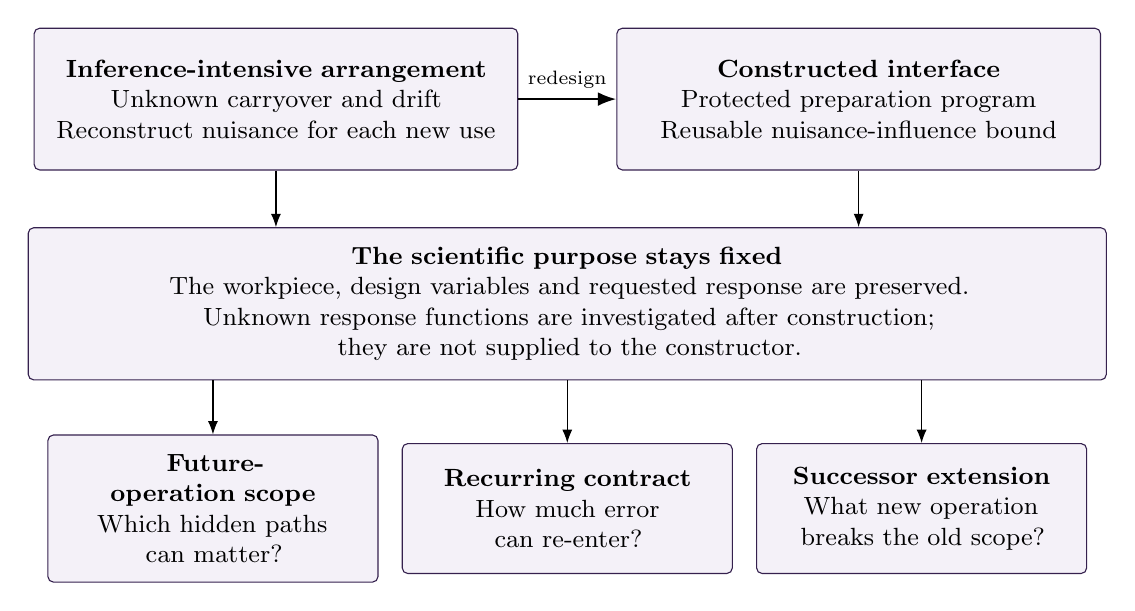
\begin{tikzpicture}[>=Latex,font=\small,box/.style={draw=ink,rounded corners=2pt,fill=pale,align=center,inner sep=7pt}]
\node[box,text width=5.65cm,minimum height=1.8cm] (old) at (0,0) {\textbf{Inference-intensive arrangement}\\Unknown carryover and drift\\Reconstruct nuisance for each new use};
\node[box,text width=5.65cm,minimum height=1.8cm] (new) at (7.4,0) {\textbf{Constructed interface}\\Protected preparation program\\Reusable nuisance-influence bound};
\draw[->,thick] (old)--node[above,font=\scriptsize]{redesign} (new);
\node[box,text width=13.2cm,minimum height=1.8cm] (purpose) at (3.7,-2.6) {\textbf{The scientific purpose stays fixed}\\The workpiece, design variables and requested response are preserved.\\Unknown response functions are investigated after construction;\\they are not supplied to the constructor.};
\draw[->] (old.south)--(purpose.north -| old.south);
\draw[->] (new.south)--(purpose.north -| new.south);
\node[box,text width=3.7cm,minimum height=1.65cm] (scope) at (-.8,-5.2) {\textbf{Future-operation scope}\\Which hidden paths\\can matter?};
\node[box,text width=3.7cm,minimum height=1.65cm] (repeat) at (3.7,-5.2) {\textbf{Recurring contract}\\How much error\\can re-enter?};
\node[box,text width=3.7cm,minimum height=1.65cm] (next) at (8.2,-5.2) {\textbf{Successor extension}\\What new operation\\breaks the old scope?};
\draw[->] (purpose.south)--(repeat.north);
\draw[->] (purpose.south -| scope.north)--(scope.north);
\draw[->] (purpose.south -| next.north)--(next.north);
\end{tikzpicture}
\caption{The output is a qualified experimental arrangement. This diagram describes the construction implemented in the reference model; it is not a deployed laboratory architecture or an autonomous discovery claim.}
\label{fig:architecture}
\end{figure}

\section{Executed construction, transfer and comparison}
\label{sec:study}
\subsection{Inputs, unknowns and actual scope}
The reference study uses Python's standard library, integer support maps and rational arithmetic. It has no model call, external service, network operation or physical actuator. The six-channel fixture and primitive catalogue are authored. The constructor receives guards, support envelopes, costs, productive-command scope and later magnitude requirements. It does not receive the nonlinear scientific response laws, realized nuisance coefficients, future query sequence or hidden values.

The exact structural fixture includes one dormant reservoir. Its productive language initially rotates only the six working channels. The exposed readout is channel zero. Backward closure therefore gives six relevant coordinates and leaves the reservoir outside the capability scope. Table~\ref{tab:structure} records actual search results. Catalogue costs are abstract resource units; no currency or equipment quotation is implied.

\begin{table}[htbp]
\centering\small
\begin{tabularx}{\linewidth}{Yrrr}
\toprule
Construction and obligation & Reachable labels & Installation + use & Operation cost\\
\midrule
Anchor-only readout protection &137&12&3\\
All declared productive words, unguided mixer &7&Infeasible&---\\
All declared productive words, directional access &137&35&18\\
Same obligation, global replacement also available &145&35&18\\
New reservoir scope, valid inherited state/modules &258&12&5\\
Expanded scope constructed from scratch &405&45&21\\
\bottomrule
\end{tabularx}
\caption{Exact structural programs in the ideal-zero model. ``Infeasible'' means no admitted construction in that complete catalogue search, not an impossibility of physical redesign. Recurrent finite-precision costs are a different qualification layer.}
\label{tab:structure}
\end{table}

The qualified structural word is
\begin{center}
\texttt{protect; drain; (route; drain)}$^{5}$\texttt{; release}.
\end{center}
It costs 17 installation units and 18 operation units. Direct rational matrix multiplication shows that every relevant initial nuisance direction is annihilated, while the dormant reservoir is retained.

Without directional access, the accepted support envelope allows the mixer to copy an uncleared neighboring signal into a cleared location. For the reference ring, a worst-case allowed row selection restores all six positive signals after each local drain. Repeated observation can reveal this behavior; it cannot turn that particular local action catalogue into a qualifying physical reset. Additional sensing-and-subtraction, stronger mixing restrictions or a different productive interface would be new, potentially valid alternatives. They are not declared defeated.

\subsection{The cost of repeatability}
The recurring magnitude parameters are
\begin{equation}
 d=6,\quad H=\frac1{50},\quad a=L=1,\quad b=\frac15,
 \quad\eta=\frac1{10000},\quad\tau=\frac1{2000},
 \quad\varepsilon=\frac1{10}.
 \label{eq:settings}
\end{equation}
All are supplied reference assumptions. They describe a bounded signal-memory model, not a measured material concentration or physical apparatus. Equation~\eqref{eq:k} gives $r_*=1/501$ and $k_*=3$.

A single-use construction uses two drains per channel. Its first worst-case error is $0.0003$, which passes. Its second worst-case error is $0.002102$, which fails. The three-drain construction instead has
\begin{equation}
 \rho=\frac1{1000},\qquad
 B=\frac1{4995},\qquad
 E=\frac{2999}{9990000}\simeq0.0003002002 <0.0005.
 \label{eq:actualbound}
\end{equation}
The bound holds for every history admitted by the contract, not merely the saved simulation. Its optimal operation cost is $2+6\cdot3+5\cdot2=30$. Repeating three full sweeps costs 50. The 40\% reduction concerns these declared operation units only; it is not a measured reduction in laboratory expense, end-to-end research time or model inference.

\begin{figure}[htbp]
\centering
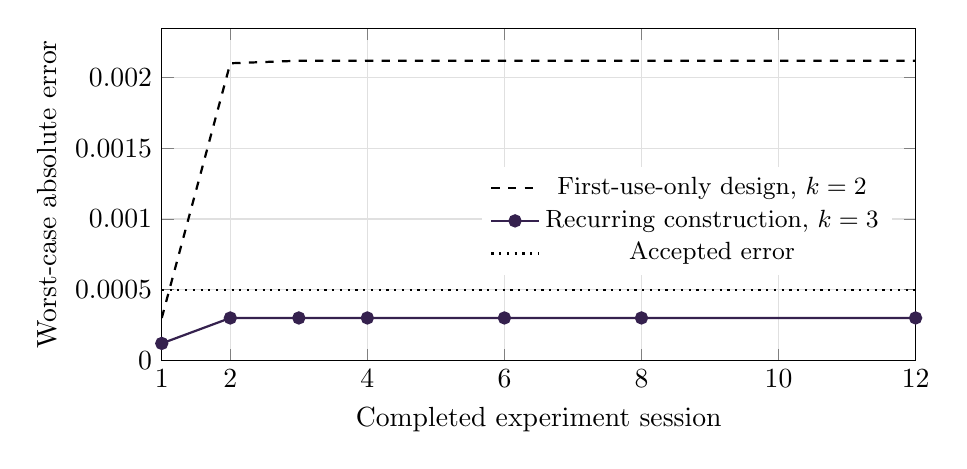
\begin{tikzpicture}
\begin{axis}[width=.92\linewidth,height=5.8cm,xlabel={Completed experiment session},ylabel={Worst-case absolute error},xmin=1,xmax=12,ymin=0,ymax=.00235,scaled y ticks=false,ytick={0,.0005,.001,.0015,.002},yticklabel style={/pgf/number format/fixed,/pgf/number format/precision=4},xtick={1,2,4,6,8,10,12},legend style={at={(.97,.42)},anchor=east,font=\small,draw=none,fill=white},grid=major,major grid style={draw=black!12}]
\addplot[black,dashed,thick] coordinates {(1,.0003)(2,.002102)(3,.00212002)(4,.0021202002)(5,.002120202002)(12,.002120202021)};
\addlegendentry{First-use-only design, $k=2$}
\addplot[ink,thick,mark=*] coordinates {(1,.00012)(2,.00030002)(3,.00030020002)(4,.00030020020002)(6,.0003002002002)(8,.0003002002002)(12,.0003002002002)};
\addlegendentry{Recurring construction, $k=3$}
\addplot[black,dotted,thick] coordinates {(1,.0005)(12,.0005)};
\addlegendentry{Accepted error}
\end{axis}
\end{tikzpicture}
\caption{Exact worst-case recurrence from the supplied contract. The first-use design passes session one and fails session two. The lower curve is bounded for arbitrarily many sessions under the stated assumptions; the finite plot is not itself the proof. Coordinates are rounded presentations of saved rational results.}
\label{fig:repeat}
\end{figure}

\subsection{Confirmation under changing, unknown nuisance dynamics}
After code and the reference construction were frozen, a new seed generated 64 synthetic campaigns of 128 sessions each. Each session used a newly generated coupled nuisance update whose row sums were at most one, a bounded new injection, unknown permitted attenuation and routing gains, and bounded readout error. The next design coordinate depended partly on the preceding reported value, so query selection was adaptive rather than a fixed list.

The simulator uses integer finite-resolution states with scale $10^9$. Each positive multiplication is rounded downward. These nonlinear rounding operations preserve the order and norm bounds required by Theorem~\ref{thm:repeat}; they are not silently described as exact real-valued matrix products. Every realized weight, injection, reset factor, pre-reset state, post-reset state, query and reported answer is saved. A second interpreter replays all 8,192 queries and 8,128 within-campaign transition links using integer arithmetic and separately recomputes the nonlinear response laws.

The greatest actual query error was $0.000157643$, below the exact bound in \eqref{eq:actualbound}. No sample failure rate is promoted to a universal performance claim. The certificate is conditional on the envelopes; the confirmation detects implementation inconsistencies and exercises varied histories within them. A scalar endpoint recurrence separately demonstrates sharpness of the general envelope, so the smaller random maximum is not used to tighten it.

\subsection{Two downstream decisions, one retained interface}
The same constructed interface is reused without changing its reset program for two $24\times24$ design studies. Let $x,y\in\{0,1/23,\ldots,1\}$. The first response is
\begin{equation}
 F_{\max}(x,y)=1-(x-7/13)^2-\tfrac32(y-5/11)^2+xy/40.
 \label{eq:response1}
\end{equation}
The second, used for inverse design, is
\begin{equation}
 F_{\mathrm{inv}}(x,y)=x^3+2y^2+\tfrac3{35}xy+\tfrac1{45}.
 \label{eq:response2}
\end{equation}
These are authored synthetic response laws. They are unknown to the constructor, not to the study author. The downstream solver must still make observations; it is not granted knowledge of a physical scientific result.

The maximization study selects grid coordinate $(13,11)$ and has zero regret against the exact finite grid. Its intervals do \emph{not} separate it from every alternative, so the operational result is the $2E\simeq0.0006004004$ regret certificate, not a certified unique optimum. The distinction is retained in the saved result.

The inverse-design study seeks response $2/3$ and selects coordinate $(2,13)$. Its actual target error is approximately $0.000632729$, while its measured-value certificate is approximately $0.000739242$, below the separately specified $0.002$ tolerance. Across the two applications, all 1,152 measured response intervals contain their exact target values.

This demonstrates a reusable enabling interface for two different decision requirements. It does not establish two independent discoveries of that interface, two physical scientific breakthroughs or two businesses. Their common gain is that neither solver must reconstruct the changing nuisance dynamics before trusting its response intervals.

\subsection{Structural diversity and ordinary competitors}
A separate fresh seed generates 96 different support systems with three to seven coordinates, four maintenance primitives, two productive primitives, module costs and exposed coordinates. Ninety-five admit a construction; one is rejected by complete reachability. The checker validates 3,034 reachable labels and 12,136 edges for these generated systems. Including the six primary/extension graphs, it validates 102 graphs, 4,123 labels and 15,251 edges. These counts describe the chosen generator, not the frequency of constructible real systems.

The classical comparison is deliberately strong within the model. Exact support search sees the same complete catalogue and matches the optimum by construction. Independent attenuation-count dynamic programming matches the local formula. A global replacement module is allowed to win when its full declared resource cost becomes lower. The experiment therefore does not attribute known planning or control capabilities uniquely to \Om.

\begin{table}[htbp]
\centering\small
\begin{tabularx}{\linewidth}{P{3.8cm}Y}
\toprule
Alternative & What the actual comparison establishes\\
\midrule
More raw observations & Can leave two different intended response laws observationally identical; a concrete algebraic alias is saved. This is an interface restriction, not a universal limitation of measurement.\\
Current-readout-only preparation & Costs 3 operation units but fails after an allowed exposing suffix.\\
Single-use precision design & Costs 24 operation units; passes the first required accuracy test and fails the second.\\
Three complete sweeps & Meets the same recurrent bound but costs 50 operation units.\\
Unrestricted local count-space planner & Matches the 30-unit optimum; no solver-superiority claim follows.\\
Qualified global replacement & Can dominate the local design at sufficiently many accepted uses under the supplied installation/operation accounting.\\
\bottomrule
\end{tabularx}
\caption{The compared claims are intentionally distinct: information, scope, repeatability, schedule cost and infrastructure choice are not collapsed into one score.}
\label{tab:comparators}
\end{table}

\section{A successor must change the interface when its purpose expands}
\label{sec:successor}
The exact primary construction leaves coordinate seven untouched. Under the original productive language, this is correct: that reservoir cannot affect any accepted operation. A new probe swaps the reservoir with the readout channel. The future-relevant set changes from six coordinates to seven, and the old claim must stop.

The constructor is given the new command support and the available protected reservoir-access primitive, not a repair recipe. It recomputes the closure and uses the valid old end-state support and already installed modules. The selected extension is
\begin{center}
\texttt{protect; expose\_reservoir; drain; release}.
\end{center}
It requires 7 new installation units and 5 operation units. From scratch, the enlarged exact capability costs 24 installation units and 21 operation units. The historical primary investment is not free: the old 35-unit campaign plus the 12-unit extension totals 47, whereas a designer who knew the enlarged scope from the start could spend 45. Succession reduces the \emph{remaining} construction burden; it need not beat advance knowledge of the final mission.

The exact failure witness sets only the dormant reservoir to one. The old prepared readout is zero; the new probe produces error one. Applying the selected extension eliminates that nuisance. This is retained-state inheritance within the same supported system, not numerical evidence copied from an unrelated plant.

For imperfect attenuation, an inherited quantitative bound can be extended only after checking the new operation's transfer and disturbance envelopes. If the old channels are bounded by $B$ and the reservoir by $H_r$, a protected swap and $k$ local drains give a new readout bound $\varepsilon^k H_r$, while the old readout moves into the reservoir with bound $B$. The extended box is bounded by $B$ when $\varepsilon^kH_r\leq B$, provided the other qualified primitives and future disturbance contract remain unchanged. That statement is an analytic extension rule; the saved successor search is the exact-support experiment, not a claim of a separately executed long-horizon quantitative successor campaign.

\begin{figure}[htbp]
\centering
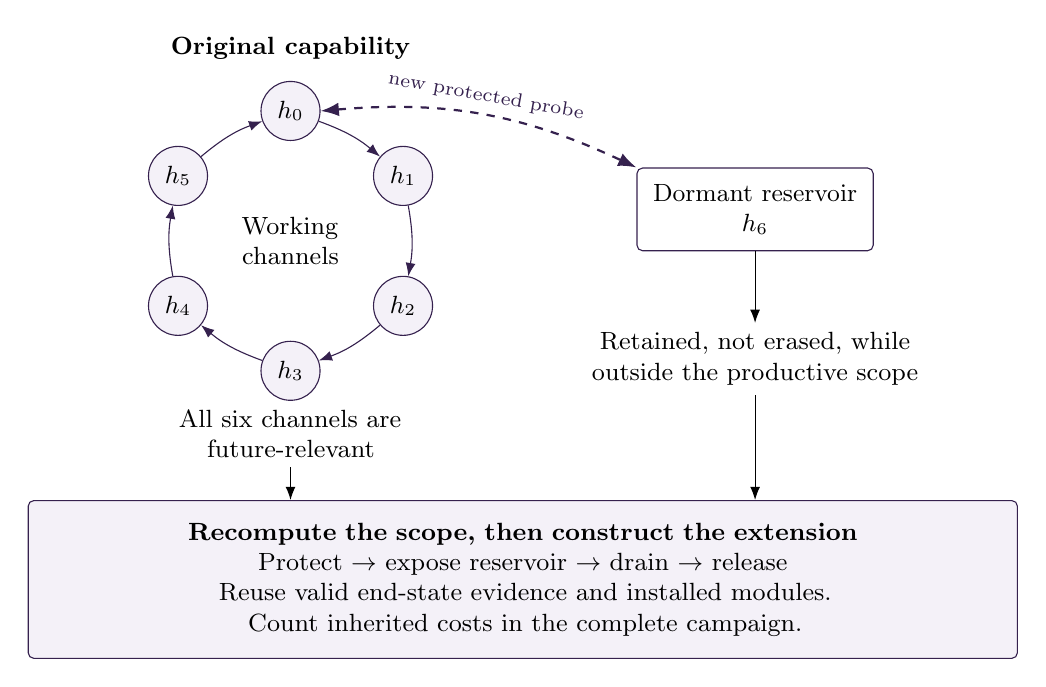
\begin{tikzpicture}[>=Latex,font=\small]
\foreach \i/\angle in {0/90,1/30,2/-30,3/-90,4/-150,5/150}{
 \node[circle,draw=ink,fill=pale,minimum size=.72cm] (p\i) at (\angle:1.65) {$h_{\i}$};
}
\foreach \i/\j in {0/1,1/2,2/3,3/4,4/5,5/0}{\draw[->,ink] (p\i) to[bend left=10] (p\j);}
\node[font=\small\bfseries] at (0,2.45) {Original capability};
\node[align=center,text width=1.8cm] at (0,0) {Working\\channels};
\node[align=center,text width=4.6cm] (scope) at (0,-2.45) {All six channels are\\future-relevant};
\node[draw=ink,rounded corners=2pt,minimum width=3cm,minimum height=1.05cm,align=center] (res) at (5.9,.4) {Dormant reservoir\\$h_6$};
\node[align=center,text width=4.3cm] (note) at (5.9,-1.5) {Retained, not erased, while\\outside the productive scope};
\draw[<->,dashed,thick,ink] (p0.east) to[bend left=15] node[above,sloped,font=\scriptsize]{new protected probe} (res.north west);
\draw[->] (res.south)--(note.north);
\node[draw=ink,fill=pale,rounded corners=2pt,align=center,text width=12cm,inner sep=8pt] (repair) at (2.95,-4.3) {\textbf{Recompute the scope, then construct the extension}\\Protect $\to$ expose reservoir $\to$ drain $\to$ release\\Reuse valid end-state evidence and installed modules.\\Count inherited costs in the complete campaign.};
\draw[->] (note.south)--(repair.north -| note.south);
\draw[->] (scope.south)--(repair.north -| scope.south);
\end{tikzpicture}
\caption{The successor introduces a genuinely new dependency. The old capability is not retroactively declared universal. Primitive access and its preservation guarantee are supplied; the repair program and its cost are computed.}
\label{fig:successor}
\end{figure}

\section{Failure is part of the capability's meaning}
\label{sec:failures}
The reference package contains explicit counterexamples rather than a registry containing only successful constructions.

\paragraph{Observations can preserve an alias.}
For all $x$, let $g_0(x)=x^2+1/3$ with nuisance $h_0=1/4$ and coupling $\ell(x)=x+1$. Let $g_1(x)=g_0(x)+(x+1)/4$ with $h_1=0$. Their raw observations are identical for every design $x$, while their intended nuisance-free responses differ. A qualifying reset exposes the difference. This algebraic example does not claim that all existing experimental methods lack an independent reference or sensor.

\paragraph{A cheap reset can destroy the purpose.}
The false solution \texttt{erase\_everything} sends a protected payload of 13 to zero. The constructor refuses it; a diagnostic run that falsely labels it preserving chooses its one-unit cost. This establishes why preservation cannot be a soft optimization reward. It does not verify that a physical interlock actually preserves the specimen.

\paragraph{Perfect-reset mathematics can misdescribe a real actuator.}
With the reference initial bound, one actual attenuation of $0.1$ leaves a first error of $0.0021$ including readout noise, while a false perfect-reset assumption would report only $0.0001$. The finite-attenuation construction is necessary; correct symbolic supports alone do not provide it.

\paragraph{A small leak can invalidate the lifetime promise.}
For the three-drain construction, the largest allowed additive reset leakage at the exact tolerance boundary is
\begin{equation}
 \delta_{\max}=\frac{499}{2500000}=0.0001996.
 \label{eq:leak}
\end{equation}
A supplied leak of $1/4000=0.00025$ raises the recurrent bound to $611/1110000\simeq0.0005504505$, exceeding the required $0.0005$. A newly widened contract can describe the result honestly; it cannot preserve the old service qualification.

\paragraph{Preparation does not create information below the readout floor.}
A requested error of $0.00005$ is incompatible with the permitted $0.0001$ readout bias even after an exact nuisance reset. A better sensor, a separately justified stochastic averaging model, a revised accepted tolerance or a different observation protocol is required. Averaging does not automatically remove adversarial bias.

\paragraph{A new productive law can defeat recurrence.}
Replacing $a=1$ with $a=1200$ makes $\rho a=1.2$. With positive repeated injection, the admitted class no longer has a finite all-history bound. Finite-horizon operation can still be evaluated. The system must not silently keep an ``indefinite reuse'' label after its stability condition changes.

\paragraph{No finite data set establishes the physical support zeros.}
A sufficiently small unmodeled path can evade finite noisy tests and later be amplified. Structural isolation must be justified by engineering, inspection or appropriate measurements and assumptions. The paper's exact support certificate and rational invariant are conditional instruments; they do not manufacture those external facts.

\section{Invent the capability and the arrangement that makes it worth building}
\label{sec:economy}
The commercial unit suggested by the construction is a \emph{qualified discovery interface}: a way to perform a declared family of useful investigations with stated accuracy, throughput, lifecycle and support obligations. A sponsor may fund its discovery and qualification; an accepted deployment purchases usable access and meaningful maintenance. Further applications can support different services or separately financed ventures. None of those relationships is created by naming them in a paper.

This applies the joint capability--arrangement perspective of \emph{Invent the Economy} \cite{boucherEconomy}. Here it also changes the technical choice before the business narrative is written. A one-use tolerance, an indefinite-use tolerance, a broader command scope and a larger committed service count can select different programs and infrastructure.

\subsection{Accepted scope changes the apparatus}
For the recurring precision settings, consider three explicitly supplied qualified technologies. The ordinary local interface has installation cost 17 and optimal per-use operation cost 30. A precision upgrade changes $\varepsilon$ from $1/10$ to $1/50$, so two drains per channel suffice; its installation cost is 42 and operation cost 24. A global replacement technology has contraction $1/10000$, installation cost 205 and per-use cost 6. Its stronger preparation is not attributed to free intelligence; it is a different assumed technology and price.

All three satisfy the same recurring magnitude contract under their supplied assumptions. Their declared technical resource costs are
\begin{equation}
 C(N)=\min\{17+30N,\ 42+24N,\ 205+6N\}.
 \label{eq:frontier}
\end{equation}
The minimum uses the local architecture for $N=1,\ldots,4$, the precision upgrade for $N=5,\ldots,9$, and global replacement for $N\geq10$. A more sophisticated local schedule is not always the right next investment.

\begin{table}[htbp]
\centering\small
\begin{tabular}{rrrrl}
\toprule
Qualified uses & Local & Precision upgrade & Global replacement & Selected\\
\midrule
1 &47&66&211&Local\\
5 &167&162&235&Precision upgrade\\
10&317&282&265&Global replacement\\
12&377&330&277&Global replacement\\
\bottomrule
\end{tabular}
\caption{Executed construction choice under supplied abstract resource accounting. Counts are scenarios, not actual purchase commitments. Prices, financing, research, integration and continuing service costs are not supplied by this table.}
\label{tab:costs}
\end{table}

Four separately constructed three-use projects cost 428 units in this model. A compatible shared twelve-use capability costs 277. The difference comes from a different infrastructure choice and shared installation, not from counting an internal transfer as new value. The example is not a newly viable business until beneficiaries actually accept terms and full lifecycle costs remain favorable. It also assumes compatible scope, rights, capacity and timing; a single apparatus cannot serve simultaneous workloads without an appropriate schedule or capacity expansion.

More generally, $C(N)=\min_i(K_i+c_iN)$ with $K_i,c_i\geq0$ is subadditive for a common supported service. To see this, take separate optimizers for $N_1,N_2$, choose the one with smaller variable cost, and reuse its installation for both groups. Its total cost is no larger than their separate totals. New scope, qualification, congestion or coordination costs can reverse the net benefit; they are not exceptions to be omitted.

\subsection{Conditional emergence, not invented demand}
Let $V_i$ be a participant's defensible benefit, $P_i$ its actually accepted payment, $A_i$ adoption cost and $\mathcal R_i$ its required allowance for risk and alternatives. Participation requires an acceptable arrangement with a positive margin relative to the relevant alternative; it cannot be inferred from an aggregate surplus. A useful local diagnostic is
\begin{equation}
 V_i-P_i-A_i-\mathcal R_i>0,
 \label{eq:participation}
\end{equation}
when these supplied quantities have consistent units and an appropriate decision interpretation.

Let $m_i$ be an accepted contribution after delivery-specific costs, $K_\theta$ the fully priced common construction for qualified design $\theta$, and $A$ genuine coordination cost. If qualification is uncertain with an independently justified probability $p$, a conditional expected-contribution test is
\begin{equation}
 \Pi(\theta)=p\sum_i m_i-K_\theta-A.
 \label{eq:profit}
\end{equation}
The equation is a supplied model, not an estimate made true by an agent. Failure costs, partial deliveries, cancellation, finance, maintenance, refunds and required reserves must be represented where relevant. This paper assigns no invented $p$ or willingness-to-pay value to its reference apparatus.

A transparent four-counterfactual test can diagnose joint emergence. For two homogeneous participants with expected delivery contribution $m$, coordinated construction cost $A$, a qualified common cost $K$ and unchanged-technology cost $K_0$, the region
\begin{equation}
 m\leq K<2m-A\leq K_0
 \label{eq:joint}
\end{equation}
permits neither a single-party version of the new construction nor coordinated funding of the old one to have positive contribution, while the joint change does. The inequalities concern a specified cost and contracting model. They do not prove an advantage over ordinary entrepreneurship, which may discover the same arrangement.

The new technical content is that $K$ and the per-use obligations are generated from a purpose scope and recurring precision requirement, rather than entered as an unexplained cheap shared core. Even so, translating an abstract operation unit into a monetary cost requires actual supplier, operator and service evidence.

\subsection{Finance the delivery path and retain the real asset}
A plan must have authorized spendable cash at every stage:
\begin{equation}
 B_t=B_0+\sum_{s\leq t}(r_s-c_s+f_s)\ \geq\ B_t^{\min}.
 \label{eq:cash}
\end{equation}
Here $r_s$ is an actual receipt, $c_s$ an actual cash cost and $f_s$ separately approved net financing, including repayments when due. Success-contingent commitments are not pre-receipt cash. Refundable funds cannot be silently used as unrestricted research capital. These are the liquidity distinctions developed in the foundation paper \cite{boucherEconomy}, not a new financing theorem.

The retained enterprise asset is the executable program, qualified hardware and bounds, scope-closure test, failure record, permitted deployment rights, customer relationships and realized cash after obligations. A growing family of scientifically useful responses does not automatically become a family of businesses: every claimed business still needs independent benefit, accepted terms and sustainable full delivery economics.

MONTREAL.AI can retain ownership of the parent while negotiating specific project licenses or separately financed application ventures. AGIJobManager's USDC route and the Alpha/Jobs v0 \$AGIALPHA routes remain distinct. Nothing here creates company equity, dividends, infrastructure ownership or a financial claim for token holders. Native settlement should earn use by improving a real service after its full burden; company success and token appreciation are different propositions \cite{boucherEconomy,boucherBrief}.

\section{What an agent system should be asked to invent}
\label{sec:agents}
The output contract changes the appropriate assignment. An agent should not be rewarded merely for proposing more experiments, invoking more agents or keeping an opaque process under increasingly elaborate supervision. It should be allowed to propose an interface whose construction reduces the knowledge required for a valuable family of outcomes, and then submit that construction to external checks.

The implemented constructor is deterministic. It can nevertheless serve as a testable component in a broader discovery system. A proposal generator can suggest protected-state boundaries, candidate operations, new measurement or isolation modules, and potential beneficiaries. A qualification process must establish the supplied semantics and reject unauthorized changes. A compiler can construct programs and expose obstructions. A separate verifier can test the claimed purpose, recurring guarantees and complete resource account. This proposed agent orchestration is not reported as an executed frontier-model campaign.

Recent work supplies relevant components and competitors. AlphaEvolve uses model-generated code and evaluation-driven search for algorithmic discovery \cite{alphaevolve}. GEPA uses execution feedback and natural-language reflection to evolve prompts and combine complementary lessons \cite{gepa}. Hyperagents makes both task-solving and meta-level modification procedures editable \cite{hyperagents}. Computer-use tools provide screenshot, mouse and keyboard interaction with configured environments \cite{computeruse}. These sources justify considering stronger proposal and execution machinery; none establishes the new construction's physical validity or the economic viability of its deployments.

A fair discovery comparison would allow a strong unrestricted agent, a control/synthesis specialist and a human engineering team to redesign the apparatus too. All must receive the same permissible operations, initial evidence, budget and authority. The relevant outcome is a newly constructed, qualified capability after discovery, verification, integration and maintenance costs, not a score that rewards the system for calling an existing reset command. The present study makes its constructor available to such a comparison; it does not invent the outcome of that comparison.

For \Om, the integration target remains one project history. Alpha would retain discovery and construction attempts. Jobs would commission bounded development and independent evaluation. Fleet would supply separately qualified execution and review. A connected interface does not itself supply a qualified apparatus, permission to spend, a customer or a valid agreement. No implementation, release, mainnet contract or repository is modified by this paper.

\section{Relationship to prior work and the inherited manuscripts}
\label{sec:related}
\paragraph{Disturbance decoupling and symbolic refinement.}
Geometric control already asks how to make outputs insensitive to disturbances; Willems and Commault provide a classical measurement-feedback treatment with stability and pole placement \cite{willems}. Feedback refinement relations formalize implementable symbolic control under set-valued dynamics and uncertainty \cite{reissig}. We do not claim that changing a system to reduce disturbance is new. Our object is an exported, purpose-closed preparation capability with guarded construction costs, a sharp recurring local schedule and an executable successor scope check. The scalar recurrence is elementary robust-control reasoning, given an explicit extremal interpretation and connected to construction.

\paragraph{Mortality, synchronization and finite compilation.}
Zero products of nonnegative matrices correspond to mortality of nondeterministic automata; shortest killing words can be exponentially long in general \cite{ryzhikov}. Kiefer and Mascle prove polynomial word bounds under joint-spectral-radius restrictions \cite{kiefer}; a September 2026 manuscript proves sharper bounds for a cycle-hub class \cite{chandelkar}. Subset and careful synchronization provide further algorithmic and complexity precedents \cite{vorel}. Our support compiler inherits this difficulty. It does not give a general polynomial-time algorithm or improve those word bounds. It adds protected modes, purpose-relative targets, module payment and a separately checked certificate to a finite reference construction. The ring's local cost theorem is a tractable special case, not a claim about every mortality instance.

\paragraph{Environment redesign.}
Planning environment redesign already treats modifications to an environment as a search object. Pozanco, Fraga Pereira and Borrajo develop a metric-agnostic approach for deterministic planning environments \cite{environment}. Our proposed category is therefore not the first instance of making the environment editable. The particular contribution is a physical/experimental contract under which unmeasured, continuously valued nuisance coefficients no longer have to be reconstructed to qualify the declared family of work.

\paragraph{The A/B/C thermal lineage.}
The first supplied thermal manuscript (A) retains latent intervention dependencies so an initially invisible bridge is not discarded. The second (B), \emph{Capability Genesis}, calibrates a reciprocal boundary response and constructs a minimal extension for new ports. The third (C) changes scalar experimental access under a stronger physical class. Their mechanisms differ; their query counts and physical assumptions are not interchangeable. Their common lesson is retained, but the new paper does not add another thermal example or import their bounds into a different observation model \cite{boucherABC}.

\paragraph{The immediate predecessor.}
\emph{Discoverability by Construction} (D) compiles additional observation functions and proves a sharp finite-ensemble recovery bound. Its unknown is a population; its primitive transition maps and fresh preparation are supplied. Here the productive response can remain unknown and nonlinear, nuisance coefficients can drift within envelopes, and a protected preparation program is synthesized. The difference is not ``more measurements.'' It is a constructive way to stop some hidden quantities from needing measurement at all. D's code was rerun in the present work: 38 tests passed and seven principal output files matched byte-for-byte. That reproduces D's computations, not a physical experiment \cite{boucherD}.

\paragraph{Transformational intelligence and economic possibility.}
The original framework separates an intended purpose from its inherited formulation and evaluator \cite{boucherTI}. The current construction preserves the purpose while changing the apparatus and workflow. \emph{Invent the Economy} makes capability, beneficiaries, rights and financing a joint object of search \cite{boucherEconomy}. The resource frontier here supplies a concrete feedback from accepted recurring scope to selected technology. A proof that such a package is internally coherent is not evidence that actual participants have accepted it.

\section{Limits, next decisive experiment and conclusion}
\label{sec:conclusion}
The positive result is an executable capability constructor with complete proofs for its model, exact resource certificates, a recurring precision construction, fresh numerical/symbolic checks and a computed successor. Its scientific significance is a specific kind of leverage: an unknown system can be made usable for a declared family of investigations without first identifying every hidden condition or coefficient.

Several boundaries are material. Structural zeros and preservation guarantees are assumed, not discovered from arbitrary noisy data. Exact finite search can be exponential. Positive magnitude envelopes can be conservative for a particular plant. The local optimality theorem is limited to the cyclic actuator architecture and its specified recurring uncertainty class. The scientific response functions and cost units are authored reference inputs. No physical carryover process, autonomous invention policy, comparative frontier-model trial, paid adoption or external peer review is claimed.

A decisive physical study would begin with an independently selected nuisance-limited instrument and retain a competent sensing-and-correction alternative. The investigator would measure or otherwise justify the protective boundary, possible transfer paths, finite attenuation, re-entry disturbances and sensor bias. The constructor would then return a qualified program or a concrete obstruction. A new scientific objective and a later interface extension would test transfer with their full costs recorded. This is the unrun next test; it is not substituted for the completed construction reported here.

The long-horizon company foundation is correspondingly specific. \Om\ should discover capabilities from which families of discoveries and businesses can grow. An early deployment should leave behind more than its result: it should leave a better instrument, a known domain of validity, an executable extension path and permitted productive rights. Later scientific, industrial and infrastructure work must earn its own qualification and financing. An accumulating civilization of such assets is an ambition, not a conclusion of a finite study.

\insight{\textbf{The next output of intelligence need not be a better description of the same difficult world. It can be a constructed part of the world that makes the next family of discoveries easier to realize.}\par\smallskip The criterion is operational: preserve what matters, remove a demonstrated obstruction, build the enabling capability, and retain evidence of what can safely and economically inherit it.}

\appendix
\section{Technical details of closure, optimality and guarantees}
\label{app:math}
\subsection{Why the productive closure is the exact structural target}
For a coordinate $j$, a nonzero term in a product $C_{c_m}A_{c_{m-1}}\cdots A_{c_1}e_j$ corresponds to a labelled path from $j$ to an exposed coordinate. With nonnegative factors, every term is nonnegative; an allowed positive path can be realized without cancellation. Therefore the union of supports of all such products is exactly the backward closure $R$ under support-complete rectangular semantics. The same statement applies to a row of $E_c$. Since the coordinate set is finite, backward expansion stabilizes after at most $d$ strict additions, and a simple exposing path uses at most $d-1$ transitions before direct exposure.

If $\mathcal C\subseteq\mathcal C'$, then $R\subseteq R'$. Thus adding future operations cannot make a nuisance coordinate less relevant. An inherited exact program remains valid precisely when its retained end support also avoids $R'$, assuming the original primitive meanings and protected-state contract remain qualified. This is a test, not permission to assume that adding hardware leaves the old dynamics unchanged.

If uncertainty instead ties coefficients across time or forbids certain simultaneous edges, the support union can admit unrealizable paths. The criterion remains conservative sufficient evidence, but its ``only if'' direction must then be replaced by reachability in the constrained model. Likewise, signed systems can have cancellation and are outside the structural necessity theorem. An empty observable scope can make doing nothing correct; the constructor is not rewarded for inventing a transformation in every case.

\subsection{What the optimality certificate proves}
Let the complete reachable graph have initial node $s_0$, nonnegative edge weights and target set $G$. A candidate value $C$ is certified by a valid path of cost $C$, a function $d$ with $d(s_0)=0$, the edge inequalities \eqref{eq:potential}, and $d(g)\geq C$ for all $g\in G$. For any path $s_0,\ldots,g$, repeated substitution gives $d(g)\leq\sum c$. Therefore every target path costs at least $C$. The certificate does not need an independently trusted Dijkstra implementation.

For infeasibility, the supplied reachable set must contain $s_0$, be closed under every admitted action and contain no target. The checker validates those conditions. In the present package, the graph is generated exhaustively. A truncated graph with a missing successor is rejected. The finite theorem and certificate concern this supplied graph; an unlisted physical module could change the answer.

\subsection{Scalar necessity and boundary cases}
Write $T=(\tau-\eta)/L>0$. With $\delta=0$, the initial and recurring conditions are
\begin{equation}
 \rho H\leq T,\qquad \frac{\rho b}{1-\rho a}\leq T.
\end{equation}
For $H,b>0$, these are equivalent to
\begin{equation}
 \rho\leq\min\{T/H,T/(b+aT)\},
\end{equation}
which is \eqref{eq:k}. Because $b>0$, the second bound is strictly below $1/a$ for $a>0$. There is no unreported unstable denominator. Equality is admitted: the advertised error is an upper bound, not a strict-success probability.

For additive reset leakage, both
\begin{equation}
 \delta\leq T-\rho H,\qquad
 \delta\leq T(1-\rho a)-\rho b
\end{equation}
must hold. Substituting the reference parameters yields \eqref{eq:leak}. If either right-hand side is negative, the selected reset is not sufficient even at zero additional leakage. If $\eta\geq\tau$, the present bounded-bias model has no positive nuisance-error allowance. If $\rho a=1$ and the additive term is zero, bounded constant trajectories are possible; this boundary is handled explicitly in the code rather than called unstable by shorthand.

\subsection{The local lower bound and possible alternatives}
At endpoint actuator gains, rotations permute coordinates and drains multiply one current coordinate by $\varepsilon$. Their product is a monomial matrix: every original coordinate has one remaining path, weighted by $\varepsilon^{n_j}$. This yields \eqref{eq:counts} exactly. The lower bound on drains does not depend on a guessed optimal word. The bound on routes follows because each unit route can expose at most one previously unvisited original coordinate at the unique drain. Batching $k_*$ drains at each visited location attains both counts.

The recurring impossibility construction uses a legal between-session matrix whose every row copies a currently maximal coordinate with gain $a$. This is a signal-memory uncertainty class, not a mass-conserving transport claim. It ensures that a smaller uniform contraction cannot be hidden by distributing weakly drained coordinates across time. For a narrower physical class, different variable per-session policies, richer sensors, nonlocal drains, parallel actuation or other hardware, the stated local optimum is not a universal lower bound. Those alternatives require a new matched comparison.

\subsection{Uniform observations and selected downstream decisions}
For finite queried designs $X$, suppose $|y(x)-F(x)|\leq E$ for every $x$, even if their selection was adaptive. If $\hat x$ maximizes $y$, and $x^*$ maximizes $F$ over the queried set, then
\begin{equation}
 F(x^*)-F(\hat x)\leq[y(x^*)+E]-[y(\hat x)-E]\leq2E.
\end{equation}
No distributional inference is involved. The result concerns the queried set, not an unexamined continuum. Inverse-design acceptance follows from the triangle inequality in \eqref{eq:inverse}. The reference maximizer's lack of a unique-winner interval is retained rather than repaired by inspecting the exact hidden response and narrowing the certified error afterward.

\section{Reproduction, inputs and actual computational accounting}
\label{app:reproduce}
\subsection{Complete artifact and commands}
The computational study uses only Python's standard library. The recorded runtime is Python 3.13.5. No account, model provider, secret, network, wallet or external system is required. From the extracted package root:
\begin{lstlisting}
python code/run_study.py --out rerun
python code/check_artifacts.py --results rerun
python -m unittest discover -s code -p 'test_*.py' -v
pdflatex -no-shell-escape -interaction=nonstopmode \
  -halt-on-error -output-directory=paper \
  paper/The_World_as_an_Output.tex
pdflatex -no-shell-escape -interaction=nonstopmode \
  -halt-on-error -output-directory=paper \
  paper/The_World_as_an_Output.tex
\end{lstlisting}
The study refuses to overwrite a nonempty output directory. The manuscript embeds all figures, numerical tables and bibliography. It does not require a network fetch, external figure, BibTeX pass or shell escape. Source, development and review records are retained in \path{provenance/} and \path{review/}. Rendered-page review is a separate production check, not a scientific experiment.

\begingroup\small\renewcommand{\arraystretch}{1.0}
\begin{longtable}{P{6.5cm}P{9cm}}
\toprule
Artifact & What it contains\\
\midrule\endhead
\path{code/construct.py} & Protected support compiler, productive closure witnesses, recurrent contract and exact local schedule.\\
\path{code/reference.py} & Separate rational matrix interpreter, full distance-certificate checker, independent count-space optimization and forward integer simulator.\\
\path{code/run_study.py} & All executed construction, confirmation, downstream, failure and resource-frontier studies.\\
\path{code/check_artifacts.py} & Replay of saved primitive factors and nuisance updates; independently expanded response laws and certified intervals.\\
\path{code/test_construction.py} & 36 test methods, including certificate mutation, guard failure, preservation, exact boundaries and failure controls.\\
\path{inputs/study.json} & Complete declared parameters, fresh confirmation seeds and abstract cost assumptions.\\
\path{results/structural_constructions.json} & Six primary/extension programs and complete reachable-distance certificates.\\
\path{results/precision_contract.json} & Rational recurrence, exact local counts, 18 independent optimality checks and leakage/instability controls.\\
\path{results/structural_confirmation.json} & All 96 generated systems, their programs or rejection and all graph certificates.\\
\path{results/adaptive_confirmation.json} & Every query, unknown update weight, injection, actuator gain, state, response and error for 8,192 sessions.\\
\path{results/applications.json} & All 1,152 downstream observations, selected designs and actual versus certified conclusions.\\
\path{results/counterexamples.json} & Raw-observation alias, anchor failure, new-reservoir failure, payload damage, recurrent failure and noise-floor obstruction.\\
\path{results/resource_frontier.json} & 100 accepted-use scenarios, all three declared technologies and excluded full-lifecycle costs.\\
\path{results/frozen_constructor.json} & Byte identities of code, configuration and compiled reference artifacts before confirmation generation.\\
\bottomrule
\end{longtable}
\endgroup

\subsection{What the test counts mean}
All 36 test methods pass. They include 150 support-image comparisons, guarded ring checks over multiple dimensions, exact closure and extension checks, destruction rejection, unknown-module and invalid-cost rejection, false infeasibility under a resource cap, three mutated certificates, recurrence boundaries and independent local optimizers. The random structural study checks 96 generated instances; the all-history theorem is not inferred from their empirical frequency.

The complete scientific driver took approximately 2.11 seconds in the recorded local environment before manuscript production and review. This is a single observed wall-clock measurement, not a matched benchmark or an end-to-end cost of discovering the theory, implementing the constructor, qualifying hardware or producing the paper. The deterministic output files, excluding environment timing, can be reproduced byte-for-byte in the same environment. Fresh-package verification is recorded separately.

\subsection{Frozen artifacts and fresh confirmation}
Development used an earlier seed and retained outputs. After testable code was complete, final structural and adaptive confirmation seeds were changed to 2026102063 and 2026102059. The constructor, configuration and primary artifacts were hashed before those generated confirmation studies ran. The same author chose the model family and confirmation procedure, so this is not an externally preregistered or blinded trial. A hash identifies bytes; it does not prove an unbiased research process or correct physical semantics.

The forward simulator rounds positive products downward on a fixed $10^9$ grid. Every realized operation remains inside its order/norm envelope, which is why the rational bound can be checked without treating binary floating-point output as a formal numerical certificate. Saved inputs allow exact replay without rerunning the compiler or trusting its hidden-state calculations. No confidence interval is assigned to a deterministic exhaustive or algebraic check.

\section{Lineage, claims and research transparency}
\label{app:claims}
\subsection{Preserved sources}
The immediate predecessor's PDF, LaTeX, code and supplied package were inspected. Its computation was rerun in a separate directory; seven principal scientific outputs matched the retained package byte-for-byte and its 38 tests passed. B's earlier full reproduction was reported by D and is not relabelled as newly rerun here. A/C's larger missing companions remain manuscript-reported. This paper does not promote their physical assumptions or older model-performance assertions into fresh evidence.

The supplied foundational PDFs and A/B/C texts are preserved. Their retained repository record is commit \texttt{b7f017e91a18adb3a79b34e03dc0158896ef7570}, dated 20 October 2026 at 13:46:15 UTC. This identifies the foundation snapshot, not the current state of a live integration. No repository write, contract action, publication, funding commitment or customer outreach was performed.

Primary literature was inspected through 20 October 2026. The source ledger records the distinction between full-text inspection, abstract/metadata inspection, official documentation and supplied manuscripts. Citations to recent agent work identify proposal/execution ingredients, not experimental baselines run in this study. The review is focused rather than exhaustive, and no external peer review, proof-assistant verification or autonomous discovery-policy improvement is claimed.

\subsection{Claim--evidence register}
\begingroup\small
\begin{longtable}{P{4cm}P{5.5cm}P{6cm}}
\toprule
Claim & Evidence & Boundary\\
\midrule\endhead
Future-closed protection & Theorem~\ref{thm:closed}; executable closure and exposing suffixes & Supplied support-complete nonnegative uncertainty; no new injection in this theorem.\\
Least resource-cost exact program & Proposition~\ref{prop:compiler}; graph closure and lower-potential certificates & Finite supplied catalogue; exponential worst-case search.\\
History-uniform query bound & Theorem~\ref{thm:repeat}; exact endpoint recurrence and rational checking & Assumed preservation, recurring magnitude and readout contracts.\\
Optimal local recurring reset & Theorem~\ref{thm:local}; independent count-space optima & Cyclic local actuator class, common reset word and declared robust service scope.\\
Transfer to different decisions & Two 576-query studies; all saved intervals checked & Authored nonlinear response laws; no physical scientific discovery.\\
Actual successor construction & New closure, computed extension, exact old-scope failure & Same qualified inherited system; new access primitive supplied; quantitative successor campaign unrun.\\
Adaptive repeated operation & Exact replay of 8,192 queries and 8,128 internal links & Synthetic finite-resolution nuisance processes within envelopes.\\
Scope changes infrastructure & Three-way cost frontier, 100 scenarios & Abstract resource units, not full costs or actual demand.\\
Newly viable business & Conditional inequalities and proposed qualified-service unit & No real acceptance, receipts, operating venture or valuation established.\\
Improved invention intelligence & Not established & Requires matched independent discovery campaigns, not one constructed instrument.\\
\bottomrule
\end{longtable}
\endgroup

\clearpage
\begin{thebibliography}{99}\small
\bibitem{boucherTI} V. Boucher. \emph{Transformational Intelligence: Learning to Change the Game}. MONTREAL.AI research manuscript, October 2026. Supplied foundation, preserved unchanged. \url{https://github.com/MontrealAI/AGI-Alpha-Agent-v0/blob/b7f017e91a18adb3a79b34e03dc0158896ef7570/docs/Transformational_Intelligence.pdf}.
\bibitem{boucherEconomy} V. Boucher. \emph{Invent the Economy: Transformational Intelligence for Creating Viable Markets}. MONTREAL.AI research manuscript, October 2026. \url{https://github.com/MontrealAI/AGI-Alpha-Agent-v0/blob/b7f017e91a18adb3a79b34e03dc0158896ef7570/docs/Invent_the_Economy.pdf}.
\bibitem{boucherBrief} V. Boucher / MONTREAL.AI. \emph{SUCCESSOR $\Omega$: The Intelligence Leverage Company. Revised Company Foundation}. Six-page business design, 20 October 2026. \url{https://github.com/MontrealAI/AGI-Alpha-Agent-v0/blob/b7f017e91a18adb3a79b34e03dc0158896ef7570/docs/SUCCESSOR_Omega_Invent_the_Economy_Business_Brief.pdf}.
\bibitem{boucherABC} V. Boucher. \emph{Capability Genesis}: supplied manuscripts A (intervention-complete instruments), B (intervention-closed instruments) and C (constructing instruments), October 2026. Complete source texts retained in the common research packet and companion sources.
\bibitem{boucherD} V. Boucher. \emph{Discoverability by Construction: Synthesizing Experimental Access, Optimal Calibration, and Successor Capabilities}. Supplied 23-page manuscript and executable companion, 20 October 2026. Preserved source and reproduction record accompany this paper.
\bibitem{willems} J. C. Willems and C. Commault. Disturbance decoupling by measurement feedback with stability or pole placement. \emph{SIAM Journal on Control and Optimization}, 19(4):490--504, 1981. \url{https://doi.org/10.1137/0319029}.
\bibitem{reissig} G. Reissig, A. Weber and M. Rungger. Feedback refinement relations for the synthesis of symbolic controllers. \emph{IEEE Transactions on Automatic Control}, 62(4):1781--1796, 2017. \url{https://doi.org/10.1109/TAC.2016.2593947}. Open manuscript: \url{https://arxiv.org/abs/1503.03715}.
\bibitem{ryzhikov} A. Ryzhikov. On shortest products for nonnegative matrix mortality. arXiv:2405.19622, revision 4, 15 June 2025; conference version RP 2024, LNCS 15050:104--119. \url{https://arxiv.org/abs/2405.19622v4}.
\bibitem{kiefer} S. Kiefer and C. N. Mascle. On nonnegative integer matrices and short killing words. \emph{SIAM Journal on Discrete Mathematics}, 35(2):1252--1267, 2021. \url{https://doi.org/10.1137/19M1250893}. Open manuscript: \url{https://arxiv.org/abs/1808.00940}.
\bibitem{chandelkar} R. Chandelkar and S. S. Chadha. Quadratic bounds for uncompletable words and matrix mortality. arXiv:2609.30817, revision 2, 28 September 2026. \url{https://arxiv.org/abs/2609.30817v2}.
\bibitem{vorel} V. Vorel. Subset synchronization and careful synchronization of binary finite automata. arXiv:1403.3972, revision 4, 15 February 2016. \url{https://arxiv.org/abs/1403.3972v4}.
\bibitem{dijkstra} E. W. Dijkstra. A note on two problems in connexion with graphs. \emph{Numerische Mathematik}, 1:269--271, 1959. \url{https://doi.org/10.1007/BF01386390}.
\bibitem{environment} A. Pozanco, R. Fraga Pereira and D. Borrajo. Generalising planning environment redesign. arXiv:2402.07799, revision 2, 14 February 2024. \url{https://arxiv.org/abs/2402.07799v2}.
\bibitem{alphaevolve} A. Novikov et al. AlphaEvolve: A coding agent for scientific and algorithmic discovery. arXiv:2506.13131, 16 June 2025. \url{https://arxiv.org/abs/2506.13131}.
\bibitem{gepa} L. A. Agrawal et al. GEPA: Reflective prompt evolution can outperform reinforcement learning. arXiv:2507.19457, revision 2, 14 February 2026. \url{https://arxiv.org/abs/2507.19457v2}.
\bibitem{hyperagents} J. Zhang, B. Zhao, W. Yang, J. Foerster, J. Clune, M. Jiang, S. Devlin and T. Shavrina. Hyperagents. arXiv:2603.19461, 19 March 2026. \url{https://arxiv.org/abs/2603.19461}.
\bibitem{computeruse} Anthropic. Computer use tool. Official Claude Platform documentation, inspected 20 October 2026. \url{https://platform.claude.com/docs/en/agents-and-tools/tool-use/computer-use-tool}.
\end{thebibliography}
\end{document}
